% Festlegung des allgemeinen Dokumentenformats
\documentclass[a4paper,12pt]{article}

% Schrift
\usepackage[T1]{fontenc}
\usepackage{lmodern}
\usepackage[utf8]{inputenc}
\usepackage[ngerman]{babel}

% Bilder
\usepackage{graphicx}
\usepackage{float}
\graphicspath{{./assets/img}}

% Variablen
% Variablen
\newcommand{\titleDocument}{Masterarbeit}
\newcommand{\subjectDocument}{StudyMap: Konzeption und Evaluierung eines
innovativen Studiengangfinders am Beispiel der OTH-Regensburg}
\newcommand*{\bildquelle}{
  \footnotesize Quelle:
}
\newcommand{\code}[1]{\noindent\ignorespaces\texttt{#1}}

% Code
\usepackage{listings}
\usepackage{color}

\definecolor{black}{rgb}{0,0,0}
\definecolor{dkgreen}{rgb}{0,0.6,0}
\definecolor{gray}{rgb}{0.5,0.5,0.5}
\definecolor{mauve}{rgb}{0.58,0,0.82}

\lstset{literate=%
    {Ö}{{\"O}}1
    {Ä}{{\"A}}1
    {Ü}{{\"U}}1
    {ß}{{\ss}}1
    {ü}{{\"u}}1
    {ä}{{\"a}}1
    {ö}{{\"o}}1
    {~}{{\textasciitilde}}1
}

\lstdefinestyle{Bash} {
  frame=single,
  language=Bash,
  aboveskip=3mm,
  belowskip=3mm,
  showstringspaces=false,
  columns=flexible,
  basicstyle={\small\ttfamily},
  numbers=none,
  numberstyle=\tiny\color{black},
  keywordstyle=\color{black},
  commentstyle=\color{black},
  stringstyle=\color{black},
  breaklines=true,
  breakatwhitespace=true,
  tabsize=3
}

\lstset{emph={\$},emphstyle=\textbf}

\lstdefinestyle{Python} {
  frame=single,
  language=Bash,
  aboveskip=3mm,
  belowskip=3mm,
  showstringspaces=false,
  columns=flexible,
  basicstyle={\small\ttfamily},
  numbers=left,
  numberstyle=\tiny\color{mauve},
  keywordstyle=\color{mauve},
  commentstyle=\color{dkgreen},
  stringstyle=\color{dkgreen},
  breaklines=true,
  breakatwhitespace=true,
  tabsize=2
}

% mehrseitige Tabellen ermöglichen
\usepackage{longtable}
\usepackage{diagbox}

% Packet für Seitenrandabstände und Einstellung für Seitenränder
\usepackage{geometry}
% Internet
%\geometry{left=3.5cm, right=2.5cm, top=2.5cm, bottom=2cm}
% Kern
\geometry{a4paper, top=27mm, left=20mm, right=20mm, bottom=35mm, headsep=10mm,
footskip=12mm}

% bricht lange URLs "schön" um
\usepackage[hyphens,obeyspaces,spaces]{url}

% Festlegung Art der Zitierung
\usepackage{csquotes}
\usepackage[style=apa, backend=biber]{biblatex}
\addbibresource{assets/literatur.bib}

% Abstand zwischen Absätze
\setlength{\parindent}{2em}
\setlength{\parskip}{1em}

% Paket für Zeilenabstand
\usepackage{setspace}
\onehalfspacing
% Kern:
% \setstretch{1.15}

% für Bildbezeichner
\usepackage{capt-of}

% für Stichwortverzeichnis
\usepackage{makeidx}

% für Abkürzungsverzeichnis
\usepackage{acronym}

% Für Phantomsection
\usepackage{hyperref}

% Für Tabellen
\usepackage{tabularx}

% Konfiguriere das Inhaltsverzeichnis
\usepackage{tocbasic}

% Anhang: PDF einfügen
\usepackage{pdfpages}

% subsubsubsection durch paragraph
\usepackage{titlesec}
\setcounter{secnumdepth}{4}
\titleformat{\paragraph}
{\normalfont\normalsize\bfseries}{\theparagraph}{1em}{}
\titlespacing*{\paragraph}
{0pt}{3.25ex plus 1ex minus .2ex}{1.5ex plus .2ex}
% Kern:
\titlespacing{\section}{0pt}{12pt plus 4pt minus 2pt}{8pt plus 2pt minus 2pt}
\titlespacing{\subsection}{0pt}{12pt plus 4pt minus 2pt}{6pt plus 2pt minus 2pt}
\titlespacing{\subsubsection}{0pt}{12pt plus 4pt minus 2pt}{4pt plus 2pt minus 2pt}

% \autoref: Subsubsection umbenennen
\addto\extrasngerman{
    \def\subsubsectionautorefname{Unterabschnitt}
}

% Titel
\title{Bachelorarbeit}

% Autor
\author{Andreas Huber}

% Datum
\date{\today}

%
% Start
% des
% Dokuments
%
\begin{document}

% Titelseite
\thispagestyle{empty}

\begin{figure}[t]
 \centering
 
\includegraphics[width=0.4\textwidth]{assets/oth/logo}
\end{figure}

\begin{verbatim}
\end{verbatim}

\begin{center}
    \Large{Ostbayerische Technische Hochschule Regensburg} \\
    \Large{Fakultät für Informatik und Mathematik}
\end{center}

\begin{verbatim}
\end{verbatim}

\begin{center}
    \doublespacing
    \textbf{\huge{\titleDocument}}\\

    \onehalfspacing

    \begin{center}
        Zur Erlangung des akademischen Grades \\ Master of Science (M. Sc.)
    \end{center}

    \begin{verbatim}
    \end{verbatim}

    \begin{doublespace}
        \textbf{\Large{{~\subjectDocument}}}
    \end{doublespace}
\end{center}

\begin{verbatim}
\end{verbatim}

\begin{verbatim}
\end{verbatim}

\begin{flushleft}
    \begin{tabularx}{\linewidth}{@{}>{\bfseries}l@{\hspace{.9em}}X@{}}
        \textbf{Vorgelegt von:} & Andreas Huber <andreas.huber@st.oth-regensburg.de> \\
        \textbf{Matrikelnummer:}& 3370380 \\
        \textbf{Studiengang:}   & Master Informatik (Schwerp. Software Engineering) \\
                                & \\
        \textbf{Erstgutachter:} & Prof. Dr. Markus Heckner \\
        \textbf{Zweitgutachter:}& Prof. Dr. Daniel Jobst \\
                                & \\
        \textbf{Abgabefrist:}   & 20. März 2024 \\
    \end{tabularx}
\end{flushleft}
\newpage

% Einverständniserklärung
\thispagestyle{empty}
\section*{Erklärung zur Masterarbeit}

\bigskip
\bigskip 
\bigskip 

\begin{enumerate}
    \item Mir ist bekannt, dass dieses Exemplar der Abschlussarbeit als Prüfungsleistung in das Eigentum der Ostbayerischen Technischen Hochschule Regensburg übergeht.
    \item Ich erkläre hiermit, dass ich diese Abschlussarbeit selbständig verfasst, noch nicht anderweitig für Prüfungszwecke vorgelegt, keine anderen als die angegebenen Quellen und Hilfsmittel benutzt sowie wörtliche und sinngemäße Zitate als solche gekennzeichnet habe.
\end{enumerate}

\bigskip 
\bigskip 
\bigskip 

\noindent Regensburg, den \today

\bigskip 
\bigskip

\noindent\line(1,0){200}
\newline
\noindent Andreas Huber
\newpage

% Römische Nummerierung
\pagenumbering{Roman}

% Inhaltsverzeichnis
\tableofcontents

% Abbildungsverzeichnis
\newpage
\phantomsection
\addcontentsline{toc}{section}{Abbildungsverzeichnis}
\renewcommand\refname{Abbildungsverzeichnis}

\listoffigures

% Tabellenverzeichnis
\newpage
\phantomsection
\addcontentsline{toc}{section}{Tabellenverzeichnis}
\renewcommand\refname{Tabellenverzeichnis}

\listoftables

% Abkürzungsverzeichnis
\newpage
\phantomsection
\section*{Abkürzungsverzeichnis}
\addcontentsline{toc}{section}{Abkürzungsverzeichnis}

\begin{acronym}[Bash]
    % \acro{bash}[Bash]{Bourne-again shell}
    % \acro{ide}[IDE]{Integrated Development Environment}
    % \acro{ldap}[LDAP]{Lightweight Directory Access Protocol}
    % \acro{lms}[LMS]{Learning Management System}
    % \acro{oth}[OTH]{Ostbayerische Technische Hochschule}
    % \acro{sd}[SD]{Standardabweichung}
\end{acronym}

% Arabische Seitennummerierung ab hier
\newpage
\pagenumbering{arabic}

% Einleitung
\section{Einleitung}\label{einleitung}
\subsection{Einleitung und Motivation}\label{einleitung-und-motivation}
Die Wahl des richtigen Studiengangs ist ein wichtiger Schritt im Leben eines jeden angehenden Studierenden. Sie legt den Grundstein für die akademische und berufliche Entwicklung und beeinflusst den individuellen Bildungsweg maßgeblich. Angesichts der Vielfalt an verfügbaren Studiengängen stehen Studieninteressierte vor einer komplexen Entscheidung, die durch eine breite Palette von Inhalten,  Schwerpunkten und Karrierewegen geprägt ist. Diese Vielzahl an Informationen kann zu Unsicherheit und Verwirrung führen, wodurch nicht selten falsche Studienentscheidungen getroffen werden. \parencite{beckmann_verbesserung_2021}

Die vorliegende Masterarbeit greift dieses weit verbreitete Problem auf und stellt einen innovativen Ansatz zur Studienorientierung vor. Das Ziel ist es, eine benutzerfreundliche, automatisch generierte Infografik-basierte Plattform zu entwickeln, die Studieninteressierte dabei unterstützt, fundierte Entscheidungen über ihren zukünftigen Bildungsweg zu treffen. Die Anwendung namens StudyMap kombiniert moderne Datenanalyse, interaktive Benutzeroberflächen und nutzerzentriertes Design, um den Orientierungsprozess zu optimieren.

\subsection{Problemstellung/Zielsetzung}\label{problemstellung-zielsetzung}
Die derzeitige Studienorientierung wird oft durch eine Informationsflut und eine begrenzte Transparenz der verfügbaren Studiengänge behindert. Häufig kennen Studieninteressierte einen Studiengang oder eine ungefähre Richtung, in die sie gehen möchten. Um ähnliche Studiengänge oder alle Studiengänge in der gewünschten Richtung zu finden, fehlt oft der Überblick. \parencite{beckmann_verbesserung_2021} Diese Unsicherheit kann zu falschen Studienentscheidungen führen, die wiederum Studienabbrüche durch Motivationsmangel zur Folge haben \parencite{heublein_ursachen_2010}.

\noindent
Die spezifischen Ziele dieser Arbeit sind:
\begin{enumerate}
\item Entwicklung eines Konzepts für einen Studiengangsfinder auf Basis einer
interaktiven Infografik-basierten Benutzeroberfläche.
\item Implementierung und technische Umsetzung des entwickelten Systems am
Beispiel der Ostbayerischen Technischen Hochschule Regensburg (OTH-Regensburg).
\item Evaluation und Validierung eines Prototypen durch Tests mit potenziellen
Nutzern und Analyse der Ergebnisse.
\item Diskussion der Stärken und Schwächen des entwickelten Systems sowie der
möglichen Auswirkungen auf die Studienberatung.
\item Die Ergebnisse dieser Arbeit sollen dazu beitragen, die
Studienorientierung für Studieninteressierte zu erleichtern und ihnen bessere
Informationen und Orientierungshilfen zur Verfügung zu stellen.
\end{enumerate}

\subsection{Gliederung der Arbeit}
Die Arbeit beginnt nach der Einleitung mit dem theoretischen Hintergrund. Es werden bereits existierende Werkzeuge und Konzepte zur Studienorientierung beschrieben und die Theorie der Anwendung von interaktiven Systemen definiert.

Anschließend folgt das Kapitel \nameref{sec:methodik}, in dem zunächst verschiedene mögliche Algorithmen zur Darstellung aller Studiengänge besprochen werden. Daran anknüpfend werden die Datenquellen für den Studiengangsfinder hinsichtlich ihrer Herkunft bzw. Beschaffung diskutiert.

Das nächste Kapitel beschreibt das Konzept des innovativen Studiengangsfinders. Zunächst wird die Hochschule Regensburg als Fallbeispiel vorgestellt, einschließlich ihrer Herausforderungen und Ziele. Im Anschluss daran wird ein Konzept entwickelt, wie das Aussehen des Studiengangsfinders sein könnte und wie die Interaktivität gewährleistet werden kann. Außerdem wird in diesem Kapitel die Datenpflege und -sicherung behandelt. Dabei wird explizit auf die Datensicherung, die Trennung von Produktiv- und Testumgebung sowie auf eine Administrationsoberfläche eingegangen.

Das fünfte Kapitel behandelt den User-centered Design Prozess. Anhand von zwei Studien wird das Konzept evaluiert und verfeinert. Die erste Studie ist eine Mockup-Studie, in der das Designkonzept des Studiengangsfinders diskutiert wird. Auf der Grundlage dieser Ergebnisse wird ein Prototyp entwickelt, mit dem eine Prototypstudie mit 40 Personen, die sich für ein Studium interessieren, durchgeführt und diskutiert wird.

Nach Abschluss der Studien wird im Kapitel \nameref{sec:implementierung-und-deployment} zuerst die Auswahl der Technologien besprochen und daraufhin die Herausforderungen, die während der Implementierung entstanden sind. Schließlich werden die erläuterten Einzelkomponenten zusammengeführt und die daraus resultierende Softwarearchitektur, unterteilt in Frontend und Backend, erläutert. Der letzte Abschnitt dieses Kapitels befasst sich mit dem Software-Deployment. Es wird gezeigt, wie das Deployment abläuft, wie getestet werden kann und wie die Software letztendlich bereitgestellt wird.

Abschließend werden im letzten Kapitel die Ergebnisse und die wichtigsten Erkenntnisse zusammengefasst. Darüber hinaus wird ein Vergleich zu anderen Tools im Bereich der Studienorientierung gezogen und ein Ausblick gegeben. Im Rahmen dieses Ausblicks werden mögliche Erweiterungen und Anwendungen für die Zukunft diskutiert.
\newpage

% Theoretischer Hintergrund und vorhandene Studiengangsfinder-Konzepte
\section{Theoretischer Hintergrund und vorhandene Studiengangsfinder-Konzepte}
\subsection{Bisheriges Vorgehen bei der Studienorientierung}
% Wahl des Studiengangs PDF Seite 355
% Hochschulinformationstage wurden von MINT-Studierenden insgesamt häufig zur Studienentscheidung und Studienplanung genutzt (72 %).

% 1. Wichtigster Faktor Fach, 2. Ort o. Hochschultyp
% Oft kennen ein Fach, danach suchen sie einen Ort bzw. eine Hochschule
% Wenn sie dann auf die OTH Seite kommen, können sie nach der Kategorie suchen
% und dann ähnliche vielleicht noch besser passende Studiengänge finden
% Wichtigster Fachwahlgrund: Begabungen und pers. Neigungen
% Was Eltern, Verwandte u. Freunde sagen nur 0,1 %
% (Seite 67 von neuem PDF)
% 5 Typen schon Entscheidern, jeder entscheidet nach Pers. Neigung -> umso
% wichtiger ist es ihnen alle ähnlichen Studiengänge zu präsentieren!

Die Studienorientierung ist ein entscheidender Schritt im Bildungsweg eines
jeden Studieninteressierten und die Entscheidung für ein zukünftiges Studienfach
und eine Hochschule wird traditionell von verschiedenen Faktoren beeinflusst.
Eine umfassende Studie von CHE und EINSTIEG aus dem Jahr 2007 gibt Einblicke in
die Präferenzen und Entscheidungsmuster von Studieninteressierten.

Die Studie zeigt, dass für einen Großteil der Befragten (87,2 \%) die Wahl der
Hochschule und des Hochschulortes weniger relevant ist als das gewählte
Studienfach \parencite{einflussfaktoren}. Dies deutet darauf hin, dass das
persönliche Interesse an einem bestimmten Studienfach die Entscheidung stärker
beeinflusst als die geografische Lage oder der Ruf der Hochschule.

Ein weiteres wichtiges Ergebnis der Studie ist, dass 64,6 \% der Befragten ihr
Studienfach nach ihren Neigungen und Begabungen wählen
\parencite{einflussfaktoren}. Dies verdeutlicht, dass persönliche Neigungen und
individuelle Fähigkeiten die Studienentscheidung maßgeblich beeinflussen.

Die Erkenntnis, dass sich Studieninteressierte bei ihrer Studienfachwahl von
unterschiedlichen Motivationsfaktoren leiten lassen, führt zu der Vorstellung,
dass es verschiedene Entscheidungstypen gibt. Intrinsische Altruisten,
heimatgebundene Hedonisten, serviceorientierte Unabhängige und leistungsstarke
Karriereorientierte sind einige der identifizierten Gruppen, die jeweils
unterschiedliche Prioritäten bei der Fach-, Hochschul- und Ortswahl setzen.
Diese unterschiedlichen Entscheidungsmuster unterstreichen die Vielfalt
individueller Studienmotivationen. \parencite{einflussfaktoren}

In der Praxis bedeutet dies, dass Hochschulen wie die OTH-Regensburg darauf
achten müssen, ihre Studiengänge ansprechend und überzeugend zu präsentieren.
Gerade dann, wenn die Hochschule als mögliche Option in Betracht gezogen wird,
spielt die Möglichkeit, das gewünschte Fach entsprechend der individuellen
Interessen darzustellen, eine entscheidende Rolle.

Ein innovativer Studiengangsfinder, der Fächer inhaltlich kategorisiert und
ähnliche Studiengänge präsentiert, könnte hier eine wichtige Rolle spielen. Mit
einer solchen Lösung könnten Studieninteressierte effektiv über Alternativen
informiert werden, insbesondere wenn der ursprünglich angestrebte Studiengang
nicht verfügbar ist. Dies trägt dazu bei, dass die Hochschule potenzielle
Studierende auch dann überzeugen kann, wenn ihre erste Wahl nicht direkt
verfügbar ist, aber dennoch ähnliche, attraktive Alternativen bietet.


\subsection{Konzepte von Studiengangsfindern}
Die Historie der Studiengangsfinder zeigt eine dominierende Tendenz hin zu
umfragebasierten Konzepten. In diesem Zusammenhang werden Studierende durch
Umfragen zu ihren Interessen, Fähigkeiten und Präferenzen befragt, um auf dieser
Grundlage Studiengangsempfehlungen zu generieren.

Umfragebasierte Studiengangsfinder vertrauen auf die subjektiven Bewertungen
der Nutzer und versuchen, durch direkte Befragungen der Studierenden ihre
Präferenzen zu ermitteln. Die daraus resultierenden Empfehlungen basieren auf
den angegebenen Interessen und Vorlieben. Jedoch sind diese Empfehlungen stark
von der Qualität der gestellten Fragen und der Interpretation der Antworten
abhängig. Um die bewusste Lenkung des Algorithmus zu verhindern, enthalten viele
Umfrage-Tools ein Minimum von 50 Fragen. Die Umfrage enthält außerdem neben
einfachen Fragen wie \glqq Interessierst du dich für Informatik?\grqq{}, sehr
allgemein gehaltene (oft private) Fragen. Intelligente Algorithmen werten dann
die Antworten auf Aussagen, wie beispielsweise \glqq Wenn ich zur Party gehe,
suche ich Kontakt mit nur wenigen, die ich kenne.\grqq{} aus und versuchen durch
Zuordnung der Charakterzüge an bestimmte Interessensgruppen, passende
Studiengänge zu finden.

Trotz ihrer weiten Verbreitung weisen umfragebasierte Ansätze gewisse
Limitationen auf. Die Ergebnisse können stark von der Selbsteinschätzung der
Studierenden beeinflusst sein, und es besteht das Risiko von Verzerrungen oder
unvollständigen Informationen.


\subsection{Theorie und Anwendung von interaktiven ähnlichen Systemen}

\newpage

% Methodik
\section{Methodik}\label{sec:methodik}
\subsection{Beschreibung der Algorithmen}
StudyMap soll Studieninteressierten einen schnellen Überblick über
alle in Frage kommenden Studiengänge ermöglichen.  Dabei soll dem Nutzer eine
interaktive Grafik präsentiert werden, mit der er anhand von Studieninhalten
(z.B. \glqq Gesundheit und Soziales\grqq{}) sofort alle relevanten Studiengänge
findet. Dazu ist es notwendig, die Studiengänge nach ihren Inhalten zu
gruppieren (Clustering) und schließlich visuell ästhetisch aufzubereiten.

Bei der Festlegung des Clustering-Algorithmus für den Studiengangsfinder wurden
verschiedene Optionen in Betracht gezogen, darunter K-Means Clustering,
Force-Directed Layouts und Multidimensionale Skalierung. Nach einer
gründlichen Abwägung der Vor- und Nachteile fiel die Wahl auf MDS. Die Gründe
für diese Entscheidung und eine Erläuterung der jeweiligen Algorithmen werden in
den folgenden Kapiteln gegeben.

\subsubsection{Force-Directed-Graphs}
Force-Directed Graph Drawing ist eine Methode zur Visualisierung von Graphen, bei der die Positionen der Knoten und Kanten aufgrund von Kräften bestimmt werden. Das Vorgehen hierbei ist vereinfacht inspiriert von Modellen der Teilchenphysik und wird häufig mit dem Verhalten von Federn verglichen. Ziel des Algorithmus ist es durch Kanten verbundene Knoten nah beinander zu platzieren und somit eine ästhetisch ansprechende Visualisierung eines Graphen zu berechnen. In \autoref{fig:force-directed-layouts} erkennt man ausgehend von einer zufälligen Positionierung (Zustand 0), eine schrittweise Optimierung der Darstellung. Wie stark oder schwach sich die Knoten jeweils \glqq anziehen\grqq{} bzw. \glqq abstoßen\grqq{} wird durch die Gleichmäßigkeit der Verteilung auf der Zeichenfläche, auch Canvas genannt, bestimmt. \parencite{schonfeld_fruchtermanreingold_2019}

\begin{figure}[H]
    \centering
    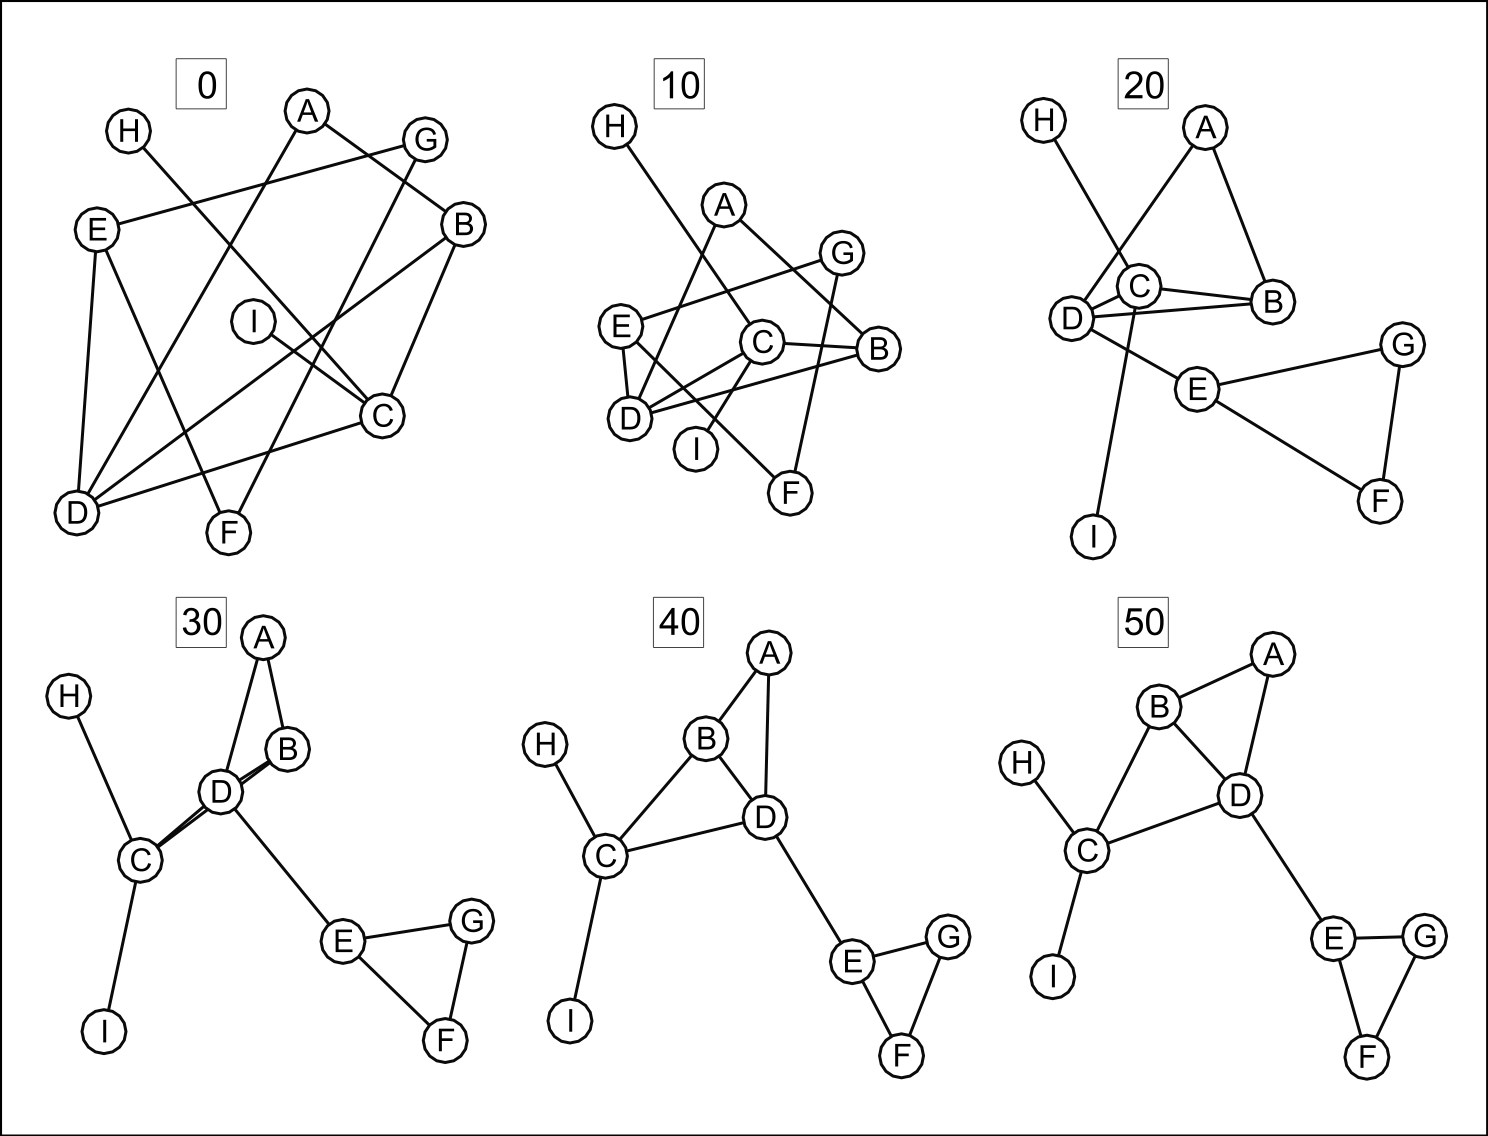
\includegraphics[width=\textwidth]{force-directed-layouts}
    \caption{Schrittweises Durchführen des Layout-Algorithmus von Fruchterman/Reingold}
    \bildquelle{Fruchterman, Thomas M. J./Reingold, Edward M.: Graph Drawing by Force-Directed Placement}
    \label{fig:force-directed-layouts}
\end{figure}

Force-Directed Layouts sind besonders effektiv für die übersichtliche
Darstellung von Netzwerken, in denen die Verbindungen zwischen den Elementen im
Vordergrund stehen. \parencite{schonfeld_fruchtermanreingold_2019} Im Gegensatz dazu
erfordert der Studiengangsfinder eine kontinuierliche Positionierung der
Studiengänge basierend auf inhaltlichen Ähnlichkeiten, was nicht unbedingt der
Stärke von Force-Directed Layouts entspricht. Force-Directed Graph Drawing
benötigt als Vorraussetzung bereits einen Graphen mit Knoten und Kanten, welche
im Fall des Studiengangsfinders die Ähnlichkeiten zwischen den einzelnen
Studiengängen entsprechen würde. Gerade die Berechnung der Ähnlichkeit zwischen
den einzelnen Studiengängen ist jedoch wesentlicher Bestandteil dieser Arbeit,
weshalb der Algorithmus nicht näher untersucht wurde.

\subsubsection{K-Means Clustering Algorithmus}
K-Means ist ein Clustering-Algorithmus, der Datenpunkte in $k$ vordefinierte
Gruppen oder Cluster einteilt. Die Wahl von $k$ stellt die Anzahl der Cluster dar,
und der Algorithmus versucht, die Datenpunkte so zu gruppieren, dass die Varianz
innerhalb der Cluster minimiert wird (siehe \autoref{fig:kmeans}).
\parencite{jeffares_k-means_2019}

\begin{figure}[H]
    \centering
    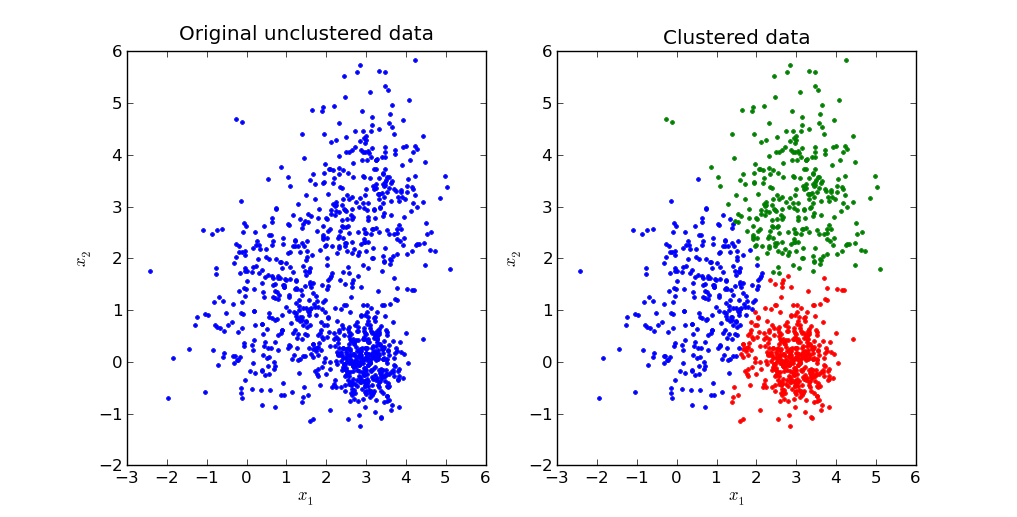
\includegraphics[width=\textwidth]{kmeans}
    \caption{K-Means Clustering Algorithmus}
    \bildquelle{https://mubaris.com/posts/kmeans-clustering/}
    \label{fig:kmeans}
\end{figure}

Die Entscheidung, den K-Means-Algorithmus nicht zu verwenden, basiert darauf, dass dieser hauptsächlich darauf abzielt, Datenpunkte zu gruppieren und weniger auf deren präzise Positionierung in einem zweidimensionalen Raum. Der Algorithmus fordert außerdem eine vordefinierte Clusteranzahl $k$. Das stellt im Falle des Studiengangsfinders jedoch keine Einschränkung dar, da jeder Cluster eine Inhaltskategorie, wie zum Beispiel \glqq Informatik\grqq{} repräsentieren würde. Dennoch ist der K-Means-Clustering-Algorithmus aufgrund seiner Empfindlichkeit gegenüber Ausreißern ungeeignet. Der Algorithmus versucht, Clusterzentren zu finden, die die Gesamtvarianz minimieren. Wenn es Ausreißer in den Studienschwerpunkten gibt, könnten sie das Ergebnis beeinflussen. \parencite{roth_demonstration_2023}

\subsubsection{Multidimensionale Skalierung (MDS)}\label{sec:MDS}
MDS ermöglicht die Reduktion $n$-dimensionaler Daten auf $m$-Dimensionen,
wodurch eine anschauliche Darstellung in Form von Koordinatenpaaren
ermöglicht wird \parencite{intro-to-multidimensional-scaling}. Dieser Aspekt ist
entscheidend, um Studiengänge in einem zweidimensionalen Diagramm zu
positionieren, wobei ähnliche Studiengänge aufgrund ihrer inhaltlichen
Ähnlichkeiten nahe beieinander liegen. Die Anwendung des MDS-Algorithmus auf
eine genormte Tabelle, in der im Falle von StudyMap die Studiengänge nach ihren
Anteilen an verschiedenen Inhaltskategorien gewichtet sind, ermöglicht eine
effektive Positionierung im Diagramm (siehe \autoref{table:input-mds}).

\begin{table}[!ht]
    \centering
    \begin{tabular}{|l|l|l|l|l|l|l|}
    \hline
        \textbf{Kürzel} & \textbf{Architektur} & \textbf{Gesundheit} & \textbf{Technik} & \textbf{Informatik} & \textbf{Wirtschaft} & \textbf{Internat.} \\ \hline
        \textbf{AT} & 0,55 & 0,06 & 0,09 & 0,04 & 0 & 0 \\ \hline
        \textbf{B} & 0,75 & 0 & 0 & 0,1 & 0 & 0,01 \\ \hline
        \textbf{ID} & 0,1 & 0,05 & 0,15 & 0,05 & 0,05 & 0 \\ \hline
        \textbf{HK} & 0,01 & 0,7 & 0,01 & 0,01 & 0,1 & 0,05 \\ \hline
        \textbf{PA} & 0 & 0 & 0,6 & 0,2 & 0,12 & 0,02 \\ \hline
        \textbf{IE} & 0 & 0 & 0,34 & 0,32 & 0,22 & 0,04 \\ \hline
        \textbf{LP} & 0 & 0,89 & 0,01 & 0 & 0,04 & 0,02 \\ \hline
        \textbf{SA} & 0 & 0,98 & 0 & 0 & 0 & 0 \\ \hline
        \textbf{IN} & 0 & 0 & 0,05 & 0,9 & 0 & 0,2 \\ \hline
        \textbf{IW} & 0 & 0 & 0,05 & 0,75 & 0,15 & 0,2 \\ \hline
        % \textbf{IM} & 0 & 0,2 & 0,1 & 0,65 & 0 & 0,05 \\ \hline
        % \textbf{BW} & 0 & 0 & 0 & 0 & 0,6 & 0,1 \\ \hline
        % \textbf{EB} & 0 & 0 & 0 & 0 & 0,5 & 0,4 \\ \hline
        % \textbf{SE} & 0 & 0 & 0,45 & 0,35 & 0,05 & 0,05 \\ \hline
        % \textbf{UI} & 0 & 0 & 0,36 & 0,12 & 0 & 0,04 \\ \hline
        % \textbf{MS} & 0 & 0 & 0,66 & 0,18 & 0 & 0,04 \\ \hline
        % \textbf{IR} & 0 & 0 & 0 & 0 & 0,1 & 0,8 \\ \hline
        % \textbf{REE} & 0 & 0 & 0,25 & 0,15 & 0,05 & 0,05 \\ \hline
        % \textbf{EI} & 0 & 0 & 0,5 & 0,25 & 0,05 & 0,05 \\ \hline
        % \textbf{ME} & 0 & 0 & 0,75 & 0,1 & 0,03 & 0,02 \\ \hline
        % \textbf{BE} & 0 & 0,07 & 0,6 & 0,12 & 0,11 & 0,06 \\ \hline
        % \textbf{MB} & 0 & 0 & 0,87 & 0,1 & 0,02 & 0 \\ \hline
        % \textbf{PT} & 0 & 0,95 & 0 & 0,03 & 0 & 0,09 \\ \hline
    \end{tabular}

    \caption{Exemplarische Eingabetabelle für den MDS-Algorithmus}
    \label{table:input-mds}
\end{table}

\autoref{table:input-mds} stellt eine stark vereinfachte Eingabetabelle für den
MDS-Algorithmus dar. Die erste Spalte enthält die Kürzel der verschiedenen
Studiengänge, wobei beispielsweise \textit{AT} für den Bachelor-Studiengang
Architektur steht. Die folgenden Spalten enthalten genormte Werte zwischen 0 und
1, die die prozentualen Anteile verschiedener Inhaltskategorien in den
jeweiligen Studiengängen repräsentieren. Diese genormten Werte werden im
n-dimensionalen Raum positioniert. Durch Anwendung des MDS-Algorithmus werden im
Verlauf die $n$-Dimensionen auf zwei Dimensionen reduziert, um schließlich eine
ästhetisch ansprechende Visualisierung in Form eines 2D-Diagramms zu generieren.

\noindent
Der klassische MDS-Algorithmus besteht aus den folgenden vier Schritten
\parencite{imperial_multidimensional_2019}:

% https://ceopedia.org/index.php/Multidimensional_scaling
\paragraph*{1. Berechnung der Distanzmatrix $ D_{ij} $}\label{sec:distanzmatrix}
Die Berechnung der Distanzmatrix $ D_{ij} $ erfolgt mithilfe des euklidischen
Abstands zwischen den Studiengängen im n-dimensionalen Raum. Der euklidische
Abstand zwischen zwei Punkten $ P_{i} $ und $ P_{j} $ wird nach der Formel

$$ d(P_i, P_j) = \sqrt{(x_i - x_j)^2 + (y_i - y_j)^2 + \ldots + (z_i - z_j)^2} $$

berechnet, wobei $ x_{i} $, $ y_{i} $, ..., $ z_{i} $ die Koordinaten von Punkt
$ P_{i} $ im $n$-dimensionalen Raum sind \parencite{ceopedia_multidimensional_2018}. Für die
Studiengangsdaten bedeutet das, dass die $n$-Dimensionen die verschiedenen
Inhaltskategorien repräsentieren.

Die euklidische Distanzmatrix $ D_{ij} $ enthält dann die euklidischen Abstände
zwischen jedem Paar von Studiengängen. In der Matrix sind die Elemente
$ D_{ij} $ die Distanzen zwischen den Studiengängen $ i $ und $ j $. Je näher
die Studiengänge in der Distanzmatrix beieinander liegen, desto näher werden sie
im finalen Diagramm platziert und umgekehrt.

Konkret in Python implementiert, sieht die Berechnung der Distanzmatrix wie
folgt aus:

\begin{lstlisting}[style=Python]
def calculate_distance_matrix(X):
    euclidean = lambda x,y:ma.sqrt(np.sum((np.array(x)-np.array(y))**2))
    D = []
    for x in X:
        tmp = []
        for y in X:
            tmp.append(euclidean(x, y))
        D.append(tmp)
    return D
\end{lstlisting}

% https://dorianhe.github.io/Intro-to-Multidimensional-Scaling/
% https://ceopedia.org/index.php/Multidimensional_scaling
% https://www.hongfeili.com/files/paper100/paper4.pdf
\paragraph*{2. Anwendung der Centering Matrix $ C $ zur Normalisierung der
Distanzen}
Die Formel $ C = I - \frac{1}{n} \vec{e} * \vec{e}^T $ berechnet die sogenannte Centering Matrix. $ I $ ist die Einheitsmatrix, $ \frac{1}{n} $ ist der Kehrwert der Anzahl der Datenpunkte und $ \vec{e} $ ist ein Vektor gefüllt mit Einsen. Das Symbol $ \vec{e}^T $ bezeichnet wie in der Mathematik üblich die Transposition des Vektors. \parencite{wickelmaier_introduction_2003}

Die Centering Matrix $ C $ wird verwendet, um die Distanzmatrix $ D $ zu
zentrieren. Das Zentrieren ist wichtig, um die Distanzen zwischen den Punkten
in der $n$-dimensionalen Raummatrix zu normieren und somit den Schwerpunkt der
Daten im Raum zu korrigieren. \parencite{wickelmaier_introduction_2003}

Schließlich wird diese eingesetzt um die Zentriermatrix $ B $ aus der
Distanzmatrix zu berechnen:
$$ B = - \frac{1}{2} * C * D_{ij} * C $$

\paragraph*{3. Spektralzerlegung}
Die Matrix $ B $ wird nun spektral zerlegt, um die Eigenwerte $ \lambda_{i} $
und die zugehörigen Eigenvektoren $ v_{i} $ zu erhalten.
$$ B = W * \Lambda * W^-1 $$
Hierbei ist $ W $ die Matrix der Eigenvektoren und $ \Lambda $ ist eine
Diagonalmatrix mit den Eigenwerten auf der Hauptdiagonale. Die Eigenvektoren
werden anschließend sortiert und die größten positiven Eigenwerte
$ \lambda_{1} ... \lambda{m} $ mit dazugehörigen Eigenvektoren
$ v_{1} ... v_{m} $ aus B extrahiert. \parencite{wickelmaier_introduction_2003}

\paragraph*{4. Projektion der Datenpunkte}
Um nun die Datenpunkte von einem höherdimensionalen Raum (basierend auf den
Beziehungen in der Distanzmatrix $ D $) auf einen niedrigdimensionalen Raum,
der durch die Eigenvektoren und Eigenwerte repräsentiert wird, abzubilden,
benötigt man folgende Projektion \parencite{he_classical_2018}:
$$ X = V_m \Lambda^{1/2}_m $$
Die Variable $ m $ steht für die Anzahl der gewünschten Dimensionen. Im Falle
von StudyMap entspricht $ m = 2 $, um das Ergebnis in einem 2D-Diagramm zu
visualisieren. $ V_{m} $ steht für die Eigenvektoren und $ \Lambda $ wie bereits
im vorherigen Absatz beschrieben für die Diagonalmatrix mit den Eigenwerten.
\parencite{wickelmaier_introduction_2003}

Abschließend enthält $ X $ die Matrix mit den auf $ m $-Dimensionen reduzierten
Koordinaten, welche dann z.B. in einem Diagramm visualisiert werden können.
An dieser Stelle wird für die Berechnung der Studiengänge (mit $ m = 2 $)
ermöglicht, dass innerhalb einer 2D-Darstellung, ähnliche Studiengänge aufgrund
ihrer inhaltlichen Ähnlichkeiten nahe beinander positioniert werden. Diese
räumliche Anordnung erleichtert die intuitive Analyse von Beziehungen zwischen
den einzelnen Bachelor- und Masterstudiengängen.

Insgesamt erfüllt der MDS-Algorithmus die spezifischen Anforderungen des
Studiengangsfinders, indem er eine übersichtliche und interpretierbare
Visualisierung der Studiengänge basierend auf inhaltlichen Ähnlichkeiten
ermöglicht.

\subsection{Beschreibung der Datenquelle und -beschaffung}
\subsubsection{Herkunft der Daten}\label{sec:herkunft-der-daten}
Die Grundlage für den Studiengangsfinder wurde in enger Zusammenarbeit mit Frau
Rösel, der Vizepräsidentin der Hochschule Regensburg, gelegt. Wir initiierten
den Prozess durch die Definition klarer Anforderungen an die benötigten
Informationen. Dazu gehört unter anderem die Definition der Inhaltskategorien
der Studiengänge. Der erste Entwurf entsprach folgender Aufteilung:

\begin{enumerate}
    \item Architektur und Bau
    \item Design und Medien
    \item Gesundheit und Soziales
    \item Technik
    \item Informatik und Mathematik
    \item Marketing und Kommunikation
    \item Erneuerbare Energien, Nachhaltigkeit und Umwelttechnik
    \item Wirtschaft und Management
    \item Internationales
\end{enumerate}

Diese Anforderungen wurden dann innerhalb der Hochschule kommuniziert und von
einer Teilmenge der Studiendekane für vereinzelte Studiengänge ausgefüllt. Das
heißt konkret, dass für 22 Studiengänge jeweils für alle dieser
Inhaltskategorien ein Wert festgelegt wurde.

Frau Rösel bleibt bis zur Übergabe der Arbeit weiterhin für die Beschaffung der Daten verantwortlich. Eine systematische Bewertung aller Studiengänge anhand des Modulplans und der jeweiligen ECTS pro Inhaltskategorie wird von Frau Rösel in Zusammenarbeit mit den Studiengangsverantwortlichen entwickelt.

Das European Credit Transfer System (ECTS) ist ein System zur Normierung von Studienleistungen innerhalb des Europäischen Hochschulraums. Dadurch können Unterschiede zwischen nationalen Hochschulsystemen ausgeglichen werden. \parencite{european_commission_europaisches_nodate} Jedes Fach an der OTH Regensburg hat eine bestimmte Anzahl von Credits (ECTS), die sich nach der Intensität des Faches richtet.

Die Bewertung des Studiengangsfinders erfolgt auf Basis der Inhaltskategorien und wird nun neutral nach der ECTS-Anzahl der jeweiligen Kategorie berechnet. So wird eine objektive Einstufung der Studiengänge für den verwendeten MDS-Algorithmus gewährleistet. Durch objektive Berechnungen ist es in Zukunft denkbar, die Aufgabe der Datenaktualisierung an eine dritte Person zu delegieren.

\subsubsection{Festlegung der Inhaltskategorien}
Im nächsten Schritt werden die Werte auf die Zeile normiert. Das heißt, die
Summe aller Inhaltskategorie-Werte pro Studiengang beträgt eins.

Im Umkehrschluss bedeutet das jedoch, dass die Studiengänge aufgrund von
Überschneidungen in den Kategorien nicht korrekt abgebildet werden können.
Beispiel:

\begin{table}[!ht]
    \centering
    \begin{tabular}{|l|l|l|l|l|}
    \hline
    \textbf{Studienfeld}           & \textbf{...} & \textbf{Informatik und Mathematik} & \textbf{Internationales} & \textbf{...} \\ \hline
    Informatik                     & ...          & 0,8                                & 0,2                      & ...          \\ \hline
    International Computer Science & ...          & 0,4                                & 0,6                      & ...          \\ \hline
    \end{tabular}

    \caption{Aufteilung der Werte bei auf Studiengang genormte Werte}
    \label{table:norm-values}
\end{table}

Tabelle \ref{table:norm-values} zeigt die Problematik der Überschneidungen. Der
Studiengang International Computer Science ist von den Inhalten nahezu
identisch zum Studiengang Informatik. Der Hauptunterschied ist, dass die Fächer
in Englisch angeboten werden. Dies hat zur Folge, dass der Studiengang
eigentlich sowohl in der Kategorie Informatik und Mathematik, als auch in der
Kategorie Internationales einen hohen Wert benötigt. Da die Zeilensumme eins
beträgt, ist dies nicht realistisch abbildbar. Aus diesem Grund wurde
entschieden die Werte pro Zelle, d.h. pro Kategorie und Studiengang auf eins
zu normieren. Mit dieser Aufteilung, kann ein Studiengang sowohl in Informatik
und Mathematik beispielsweise einen Wert von 0,8 haben, als auch in der
Kategorie Internationales.

Die anfängliche Kategorisierung der Studiengänge in neun allgemeine
Inhaltskategorien stellte sich als unzureichend heraus, da nach der Anwendung
des MDS-Algorithmus viele Studiengänge überlappend dargestellt wurden. Diese
Herausforderung führte zu einer entscheidenden Überarbeitung des
Kategorisierungssystems, um präzisere und differenzierte Bewertungen zu
ermöglichen. Die Lösung bestand in der Einführung von sogenannten Supergruppen,
die eine tiefere Bewertung der Studiengänge ermöglichten.

Ursprünglich waren Studiengänge wie \textit{Architektur} und
\textit{Bauingenieurwesen} in einer einzigen Kategorie
\textit{Architektur und Bau} zusammengefasst. Die Neuerung bestand darin, diese
in separate Kategorien wie \textit{Architektur} und \textit{Bau} zu unterteilen.
Ein zusätzliches Feld in der Eingabedatei legte fest, welche dieser Kategorien
später in der Benutzeroberfläche zu einer Supergruppe zusammengeführt werden
sollten. Dieser Ansatz ermöglichte eine präzisere Bewertung von Studiengängen,
insbesondere bei Studiengängen wie \textit{Architektur} und
\textit{Bauingenieurwesen}. Hier konnte der Studiengang \textit{Architektur} als
mehr \textit{Architektur} und weniger \textit{Bau} bewertet werden, während es
bei \textit{Bauingenieurwesen} genau umgekehrt war. Vor dieser Anpassung konnte
nur ein Wert für \textit{Architektur und Bau} festgelegt werden.

Um die Benutzeroberfläche übersichtlich zu halten, wurden Supergruppen
eingeführt. Diese ermöglichen eine aggregierte Darstellung mehrerer Kategorien,
ohne die Benutzeroberfläche unnötig zu komplex zu gestalten. Frau Rösel brachte
entscheidende Impulse in diesen Prozess ein. Durch ihre Rückmeldung wurden
darüber hinaus neue Kategorien wie \textit{Sprachkompetenzen},
\textit{Digitalität} und \textit{Future Skills} eingeführt. Diese dienen dazu,
eine noch präzisere Differenzierung und Bewertung der Studiengänge zu
ermöglichen. Folgende Liste zeigt die neuen Kategorien - jeder Listeneintrag
enthält dabei eine Supergruppe mit einem oder mehrere Kategorien:

\begin{enumerate}
    \item Architektur, Bau (Architektur und Bau)
    \item Design, Medien (Design und Medien)
    \item Gesundheit, Soziales (Gesundheit und Soziales)
    \item Maschinenbau, Elektrotechnik (Technik)
    \item Informatik (Informatik)
    \item Naturwissenschaften, Mathematik (Naturwissenschaften und Mathematik)
    \item Marketing, Kommunikation (Marketing und Kommunikation)
    \item Erneuerbare Energien, Umwelttechnik (Erneuerbare Energien und
    Umwelttechnik)
    \item Nachhaltikeit (Nachhaltigkeit)
    \item Wirtschaft, Management (Wirtschaft und Management)
    \item Sprachkompetenzen (Sprachkompetenzen)
    \item Digitalität (Digitalität)
    \item Future Skills (Future Skills)
\end{enumerate}

Die neuen Kategorien, ergänzt durch die Einführung der Supergruppen, schaffen
eine optimierte Grundlage für den MDS-Algorithmus. Dieser kann nun Studiengänge
präziser positionieren, da die Unterscheidungen und Bewertungen auf einer
feineren Ebene vorgenommen werden. Diese Anpassungen tragen entscheidend dazu
bei, das Ziel einer verfeinerten Studienorientierung und -wahl zu erreichen.
\newpage

% Konzept und Umsetzung an der OTH-Regensburg
\section{Konzept und Umsetzung an der OTH-Regensburg}

\subsection{Vorstellung der OTH-Regensburg als Fallbeispiel}

\subsection{Konzept für eine automatisch generierte Infografik}

\subsection{User-centered Design Research: Mockup eines Prototypen}

\subsection{Beschreibung der Positionsberechnung der Infografik}

\subsection{Technische Details zur Umsetzung}

\subsection{Anwendung des entwickelten Systems auf die Studiengänge der OTH-Regensburg}
\newpage

% Evaluierung und Validierung
\section{Evaluierung und Validierung}

\subsection{Beschreibung der Evaluationsmethoden und -kriterien}

\subsection{Durchführung von Tests mit potenziellen Nutzern}

\subsection{Analyse der Ergebnisse aus den Tests}

\subsection{Diskussion der Stärken und Schwächen des Systems}
\newpage

% Diskussion und Ausblick
\section{Diskussion und Ausblick}

\subsection{Zusammenfassung der Ergebnisse und wichtigsten Erkenntnisse}

\subsection{Vergleich mit ähnlichen Studienorientierungs-Tools}

\subsection{Potenzielle Erweiterungen und zukünftige Anwendungen}
\newpage

% Römische Nummerierung
\newpage
%\pagenumbering{Roman}
%\setcounter{page}{5}

% Literaturliste soll im Inhaltsverzeichnis auftauchen
\newpage
\phantomsection
\addcontentsline{toc}{section}{Quellenverzeichnis}
% Literaturverzeichnis anzeigen
\renewcommand\refname{Quellenverzeichnis}
\printbibliography
% \bibliography{assets/literatur}

% Anhang
\newpage
\phantomsection
\appendix
\section*{Anhang}
\markboth{Anhang}{}
\addcontentsline{toc}{section}{Anhang}
\renewcommand{\thesubsection}{\Alph{subsection}}

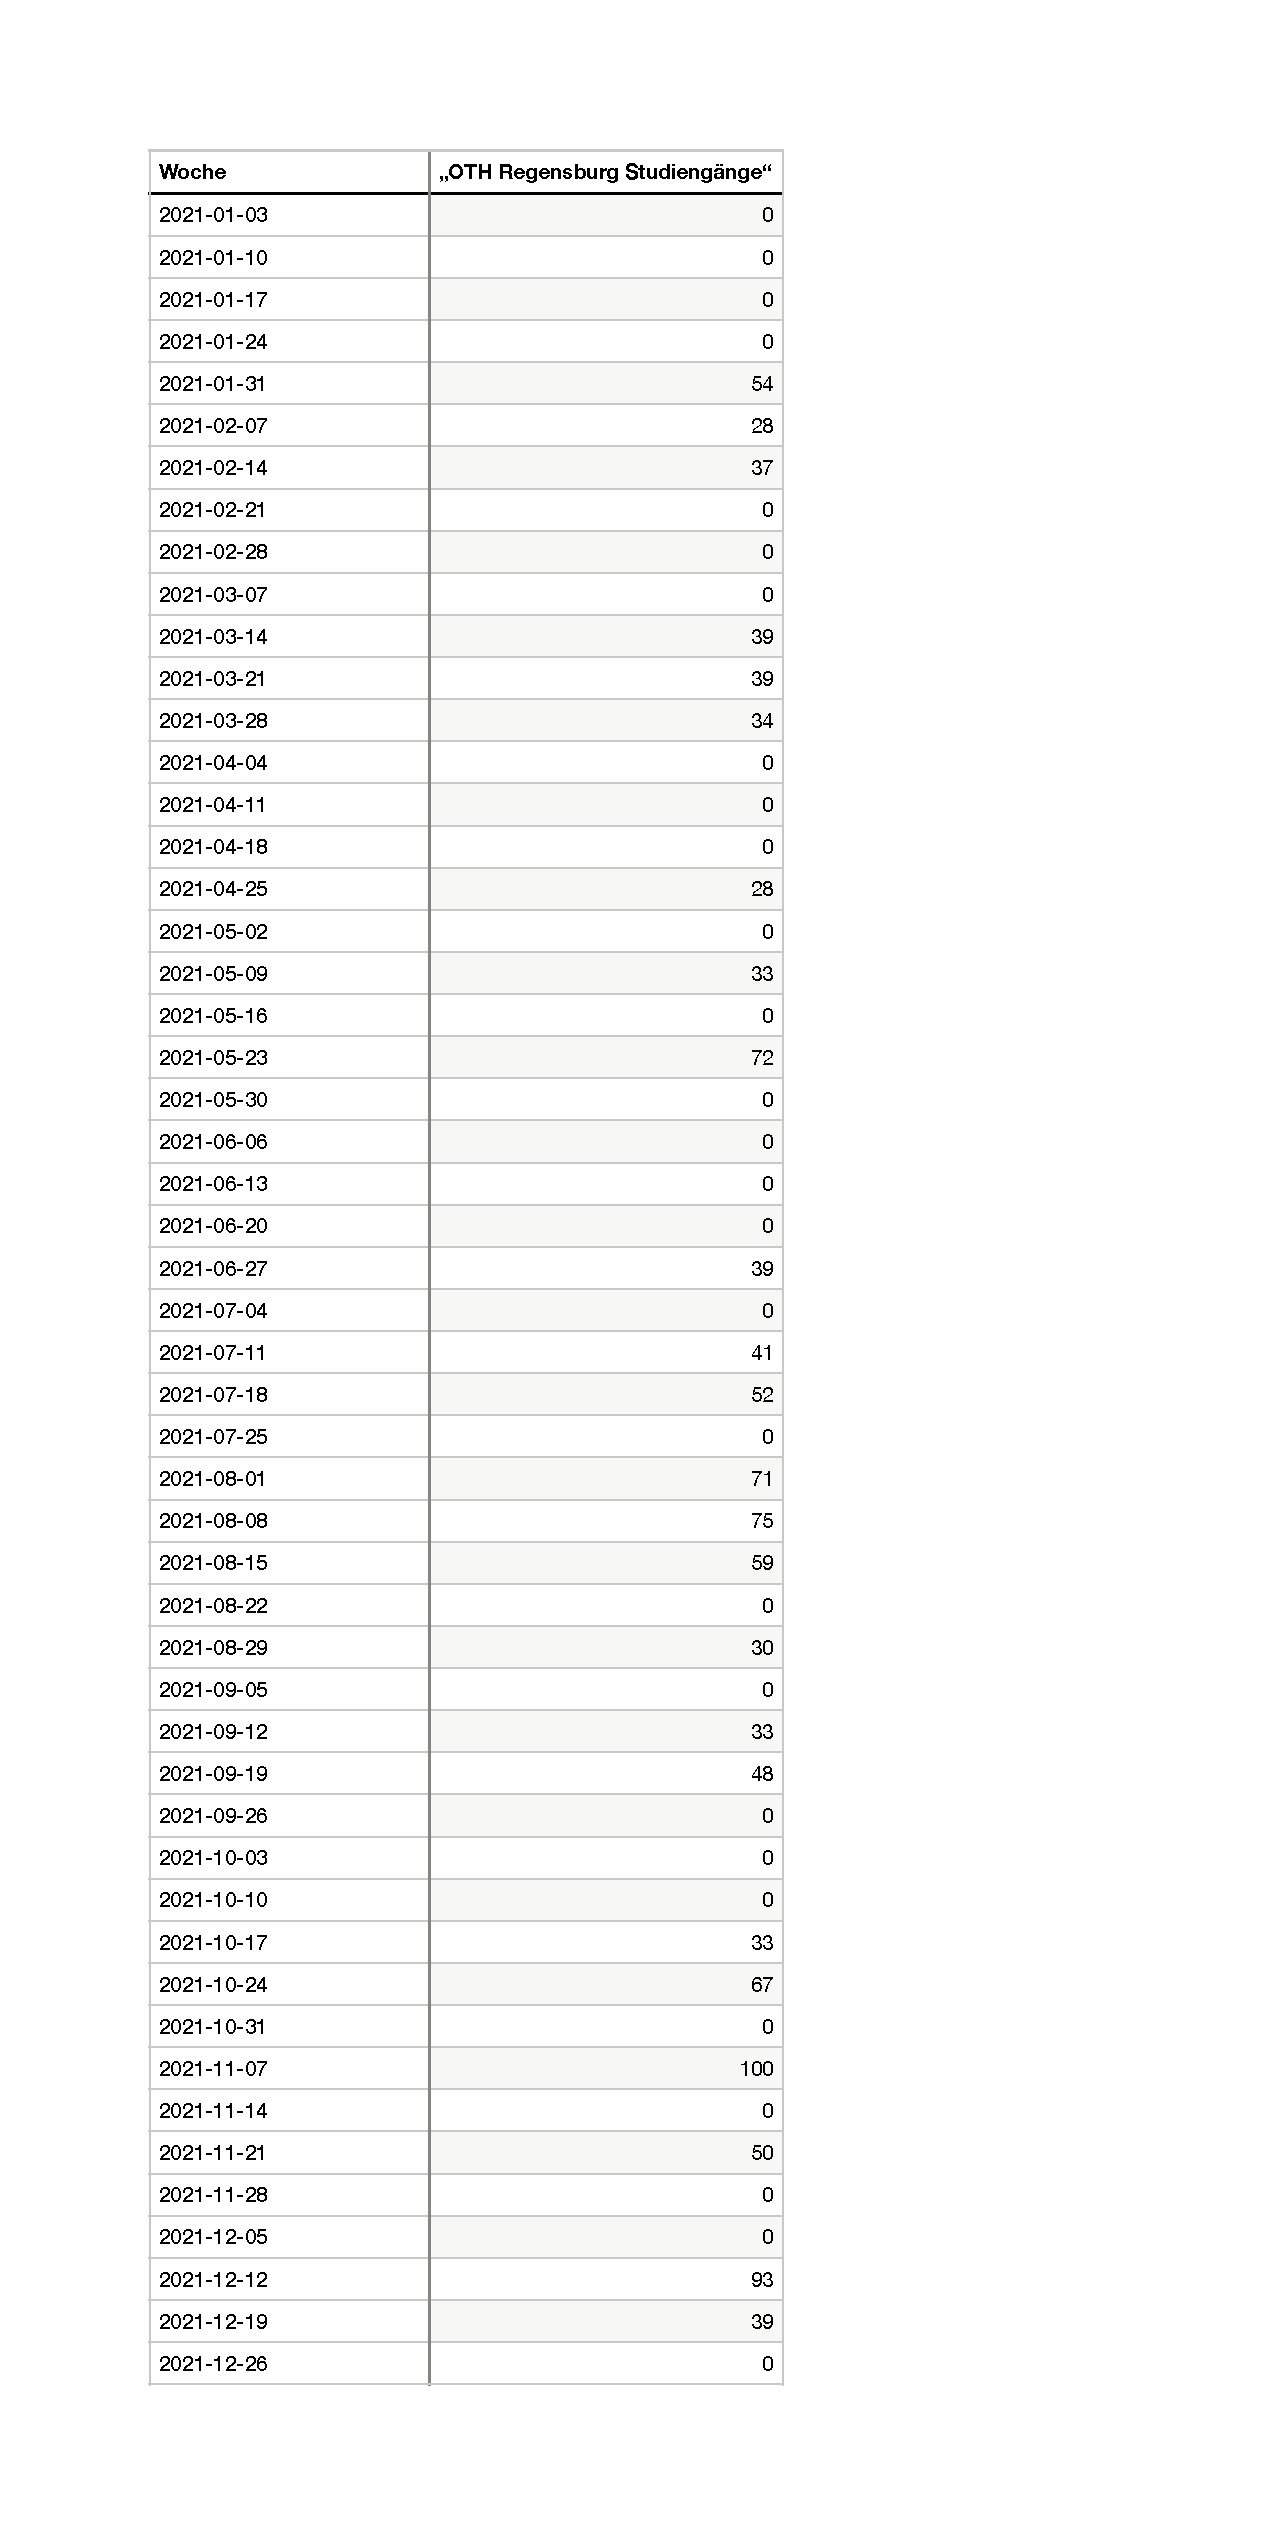
\includepdf[
    clip=0mm 0mm 0mm 0mm,
    trim=0mm 0mm 55mm 0mm,
    pages=1,
    frame,
    scale=.75,
    pagecommand=\subsection{Google Search Trends 2021: \glqq OTH Regensburg Studiengänge\grqq{}}\label{appendix:google-search-trends}
 ]{assets/pdf/google-search-trends.pdf}

\end{document}